\section{Anwendung der Methodik auf die theoretischen Grundlagen}

\subsection{Prototypische Implementierung der Integrations- und Bereitstellungs-Pipelines}
\subsection{Evaluation der Integrations- und Bereitstellungs-Pipelines unter Anwendung des Analytischen Hierarchieprozesses}
\label{sec:AHP}
Als Entscheidungsalternativen werden CI/CD-Pipelines für die Bereitstellung von Cloud-Software gegenübergestellt. Konkret handelt es sich hierbei, um die Tools \textit{SAP CI/CD}, \textit{Jenkins}, sowie \textit{Azure Pipelines}. Die Evaluation beschränkt sich dabei auf diese CI/CD-Pipelines, da diese zur Bereitstellung von Cloud-Software von der als SAP Best Practice definiert werden. Bei der Untersuchung der Pipelines müssen dabei verschiedene Aspekte beachtet werden. Zum einen soll die Pipeline auf Eignung zur Bereitstellung von auf Composable-Enterprise-Architektur basierender Software untersucht werden. Darüber hinaus muss evaluiert werden, wie gut sich die Tools für die Technologien SAP CAP bzw. SAP UI5 sowie für eine Bereitstellung auf der Laufzeitumgebung Cloud-Foundry der SAP Cloud-Plattform eignet. Diese Pipelines.
\subsubsection{Festlegung der AHP-Entscheidungsalternativen}
 Die zur Durchführung des AHP-Verfahrens benötigten Daten werden neben  Literaturrecherche ebenfalls mittels Experteninterviews erhoben. Zur Durchführung der Interviews wurde eine Expertengruppe aus X Mitarbeitenden der SAP zusammengestellt. Diese sind jeweils in spezifischen Bereichen der Cloud-Fullstack-Entwicklung, Test-Management, sowie DevOps spezialisiert. Diese umfassende Auswahl erlaubt es Expertise über verschiedene Fachbereiche hinweg zu gelangen und Anforderungen aller an der Entwicklung, Bereitstellung sowie Betrieb von Software beteiligten Stakeholdern zu erheben. Die in den Experteninterviews erhobenen Daten werden dabei ebenfalls zur Festlegung der Entscheidungskriterien verwendet. Dafür wurde eine induktive Kodierung der Expertengespräche vorgenommen. Aus besonders häufig von Experten genannten Aspekten systematisch Kategorien abgeleitet. Diese Kategorien wurden dabei ebenfalls als Entscheidungskategorien im AHP-Verfahren wiederverwendet. Da die CI/CD-Pipelines im Rahmen dieser Arbeit insbesondere für Kundenprojekte evaluiert werden, stellten sich die praktischen Projekterfahrungen der Experten als geeignete Datenquelle zur Festlegung der Entscheidungskriterien dar. Somit konnte evaluiert werden, aus welchen typischen Komponenten die CI/CD-Piplines in Kundenprojekten besteht bzw. welche Anforderungen an diese gestellt werden. Da innerhalb dieser Kundenprojekte oft weniger strikte Qualitätsanforderungen an den CI/CD-Prozess gestellt werden, wurde darüber hinaus erarbeitet, welche internen Bestimmungen, von der SAP zur Bereitstellung von Standardsoftware definiert werden. Obwohl diese Standards nur in wenigen Kundenprojekten Anwendung finden, ermöglicht ihre Berücksichtigung die Erfassung von Entscheidungskriterien, welche für eine optimale CI/CD-Pipeline erforderlich sind. Um eine effektive und klare Entscheidung treffen zu können, sollten im AHP-Verfahren ebenfalls Aspekte verglichen werden, bei sich die Entscheidungsalternativen besonders unterscheiden. Dafür wurde mittels Literaturanalyse sowie Konsultation von Online-Blogs Unterschiede der zu vergleichenden Pipelines erarbeitet. Falls es sich in einem spezifischen Anwendungsfall eignet, wurden aus diesen Erkenntnissen ebenfalls Entscheidungskriterien abgeleitet.\\
 Die mit dieser Vorgehensweise erarbeiteten Entscheidungsalternativen sind folgender Abbildung zu entnehmen. Auf der obersten Ebene des AHP-Entscheidungsbaums werden neun Kategorien definiert. Das erste Kriterium ist die \textbf{Funktionalität}. Diese Kategorie umfasst verschiedene innerhalb des CI/CD-Workflows benötigte funktionale Anforderungen. So sollte die Pipeline etwa dazu in der Lage sein, Anwendungen zu testen, Code-Analysen durchzuführen und eine Software bereitzustellen auf der Cloud-Plattform bereitzustellen bzw. für Endanwender freizugeben. Experte 1 begründet dabei, dass es bei \enquote{CI/CD-Pipelines eine Unterstützung dieser Stufen benötigt, um eine effiziente Bereitstellung von Software zu ermöglichen.} Angesichts der Komplexität der Funktionalität, wird eine Untergliederung in verschiedene Subkriterien vorgenommen. Dies ermöglicht einen präziseren Vergleich der verschiedenen Pipelines. Die hierarchische Struktur gewährleistet dabei ebenfalls ein Rahmenwerk zu definieren, welches Unterschiede in den Wichtigkeiten der Funktionalitäten berücksichtigt. In Kategorie 1.1 wird evaluiert, welche verschiedenen Tests von der Pipeline ausgeführt werden können. Die von der SAP definierten Produktstandards stützen sich dabei auf \textit{ISO 9001}, eine internationale Norm für Qualitätsstandards. Diese Norm schreibt vor, dass jede an den Endbenutzer bereitgestellte Funktionalität erfolgreich getestet wird. Im Zusammenhang mit der Softwareentwicklung bedeutet dies, dass entwickelte Features kontinuierlich und automatisiert getestet werden sollten. In Kategorie K1.1 wird dabei evaluiert, ob die zu untersuchenden CI/CD-Pipelines Backend-Tests für SAP CAP Node sowie Frontend-Tests für SAP UI5 unterstützten. Das SAP-Qualitätsmanagement schreibt für CAP-Node-Anwendungen dabei vor, dass Unit-Tests mit Jest bzw. Mocha und Integration-Tests sowie Functional-Tests mit Newmann durchgeführt werden müssen. Für SAP UI5 werden Unit-Tests mit Q-Unit, Integration sowie Functional-Tests mit OPA5 und E2E-Tests mit WDI5 vorgegebenen. Während die Test-Frameworks Jest, Mocha, Newmann sowie Q-Unit in einer herkömmlichen Node-Laufzeitumgebung ausgeführt werden, benötigt es für OPA5 sowie WDI5 einer emulierten Browser-Umgebung. Die von dem Emulator generierte Benutzeroberfläche ermöglicht das Simulieren und Testen von gezielten Anwenderinteraktionen, wie z.B. das Ausfüllen von Formularen bzw. das Klicken auf Schaltflächen. Bei der Bewertung soll dabei insbesondere evaluiert werden, ob neben der Node-Laufzeitumgebung ebenfalls eine emulierte Browser-Umgebung von den zu vergleichenden Pipelines unterstützt wird. 
In Kriterium K1.2 wird die Unterstützung verschiedener \textbf{Code-Analyse-Tools} untersucht. Dabei wurde eine bewusste Trennung dieser Kategorie mit der Kategorie der Tests vorgenommen. Während Tests eine funktionale Erfüllung der Anforderung evaluieren werden mit Code-Analysen Qualitätsstandards der entwickelten Features untersucht. Dabei wird evaluiert, ob statische Codeanalysen, Security-, Performance- sowie Code-Codepage-Überprüfungen in der CI/CD-Pipeline ausgeführt werden können. Für statische Code-Analysen werden von der SAP dabei Lint sowie SonarQube vorgeschlagen. Mit diesen Tools können neben syntaktischen Formqualitätsüberprüfungen ebenfalls Code-Metriken wie Komplexität oder Quellcode-Duplikate analysiert werden. Zur Analyse der Sicherheit wird für SAP CAP Node Checkmarx bzw. für SAP UI5 DASTER verwendet. Diese Tools sind dabei insbesondere für Composable-Enterprise-Architekturen essenziell. Da die einzelnen modularen Komponenten dieser Anwendungen insbesondere über APIs kommunizieren, bieten diese Anwendungen eine größere Angriffsfläche. Checkmarx bietet dabei verschiedene API-Sicherheitsüberprüfungen, welche z.B. auf unzureichende Autorisierung und Authentifizierung überprüfen. Auch die Open-Source-Überprüfungen helfen CEs dabei die von externen Anbieter bezogenen PBCs auf Sicherheitsrisiken zu überprüfen. Während für Performance-Tests von der SAP das Tools JMeter vorgeschlagen wird, gibt es bezüglich der Code-Coverage-Checks keine spezifische Vorgabe.\\
In der Kategorie K1.3 werden die \textit{Build-Funktionalitäten} der CI/CD-Pipelines evaluiert. 
Um Anwendungen in die Cloud Foundry Laufzeitumgebung der SAP BTP bereitzustellen wird i.d.R. das Mulit-Target-Application-Konzept (MTA-Konzept) verwendet. Die MTA ist eine Applikation, z.B. ein Microservice eines CEs, welche aus verschiedenen Modulen besteht. Diese Module umfassen typischerweise die durch ein Microservice bereitgestellte API oder eine von der Applikation verwendete Datenbank sein. Eine CE-Anwendung kann dabei ebenfalls von verschiedenen externen Ressourcen abhängig sein. Diese sind in einem Artefakt-Repository verwaltete externe Komponenten, welche bei der Entwicklung neuer Microservices wiederverwendet werden können. Diese Komponenten werden während des Build-Prozesses aus den Repositorys geladen. Darüber hinaus können die von einer CI/CD-Pipeline bereitgestellten Anwendungen ebenfalls als wiederverwendbare Komponenten in ein Artefakt-Repository eingelagert werden.
\begin{center}
	\begin{figure}[H]
		\centering
		\scalebox{0.3}{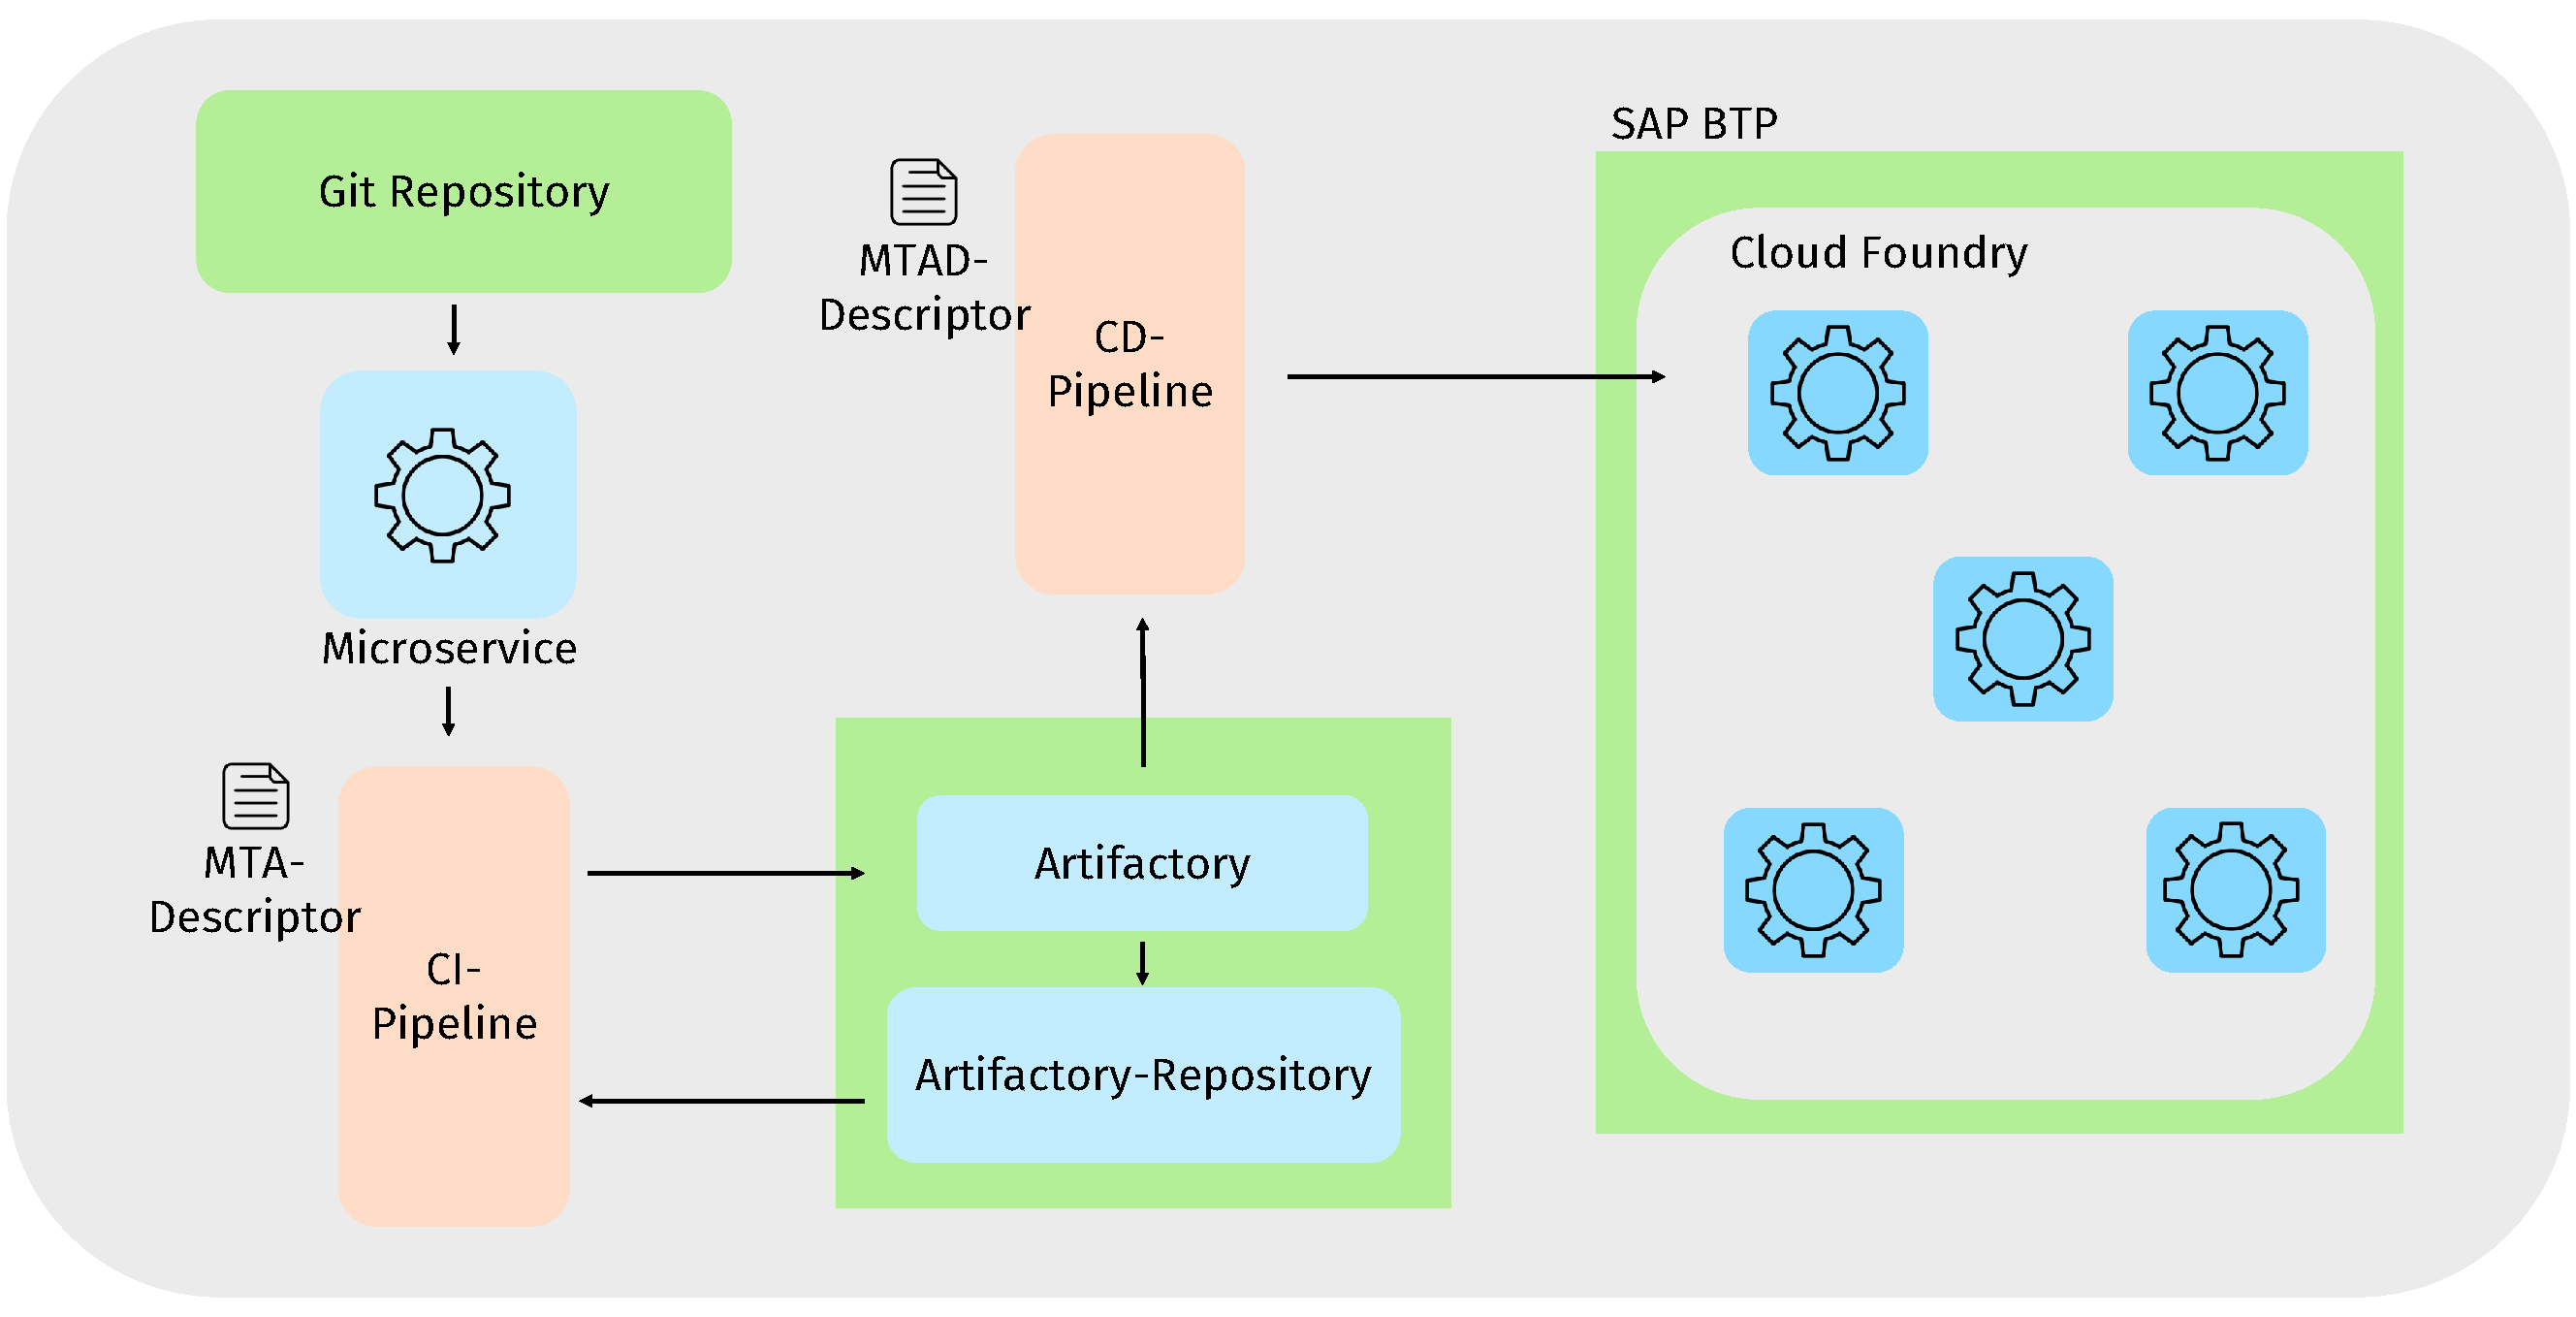
\includegraphics{MTA}}
		\caption[Bereitstellung von MTA-Applikationen in ein Artefakt-Repository]{Bereitstellung von MTA-Applikationen in ein Artefakt-Repository. Eigene Darstellung.}
		\label{fig:MTA}
	\end{figure}
\end{center}
\vspace*{-10mm}
Weiterhin ist es für eine CEA vorteilhaft, wenn ein CI/CD-Pipeline Docker-Workflows unterstützt. Mit der Hilfe von Docker-Containern können Entwickler schnell virtualisierte Umgebungen mit benötigten Frameworks und Tools einrichten ohne dabei eine gesamte Infrastruktur manuell konfigurieren zu müssen. Innerhalb des Bewertungskriteriums K1.3 wird deshalb evaluiert, Build-Tools für MTA-Anwendungen, die Verwendung von Artefakt-Repositorys sowie Docker-Workflows unterstützt.\\
Im Kriterium 1.4 (Deploy und Release) werden die Deploy- und Release-Prozesse der CI/CD-Pipelines untersucht. Dabei wird neben der Unterstützung verschiedener Bereitstellungsstrategie, ebenfalls die Integrierbarkeit in das \ac{SAP CTM} evaluiert. Dabei wird evaluiert, ob die CI/CD-Pipelines verschiedene Bereitstellungsstrategien (z.B. Blue/Green-Deployment s. Kap. \ref{sec:Bereitstellungs_Strategien}) unterstützen. Diese ermöglichen die in CEA benötigte Flexibilität und Agilität. So können neue Anwendungsversionen schnell und ohne Auswirkungen auf die Produktivsysteme bereitgestellt und getestet werden. Des Weiteren wird erörtert, ob die CI/CD-Pipelines eine Bereitstellung in das \ac{SAP CTM} unterstützten. Das SAP CTM kann als zusätzliche Schicht im CI/CD-Prozess verbaut werden. Mit dem SAP CTM können Anwendungsartefakte zwischen verschiedenen Accounts der SAP BTP verschoben werden. So könnte ein Unternehmen jeweils einen Account für die Entwicklung (DEV),für das Testen (TEST) und für die Produktionsumgebung besitzen. Mit dem SAP CTM können dabei Anwendungsartefakte im Laufe des Entwicklungsprozesses von der DEV- über die TEST- bis hin zur PROD-Umgebung transportiert werden. Dieses Delivery-System ermöglicht dabei, dass Transparenz über die Änderungsprozesse der Produktionssysteme geschafft wird. Darüber hinaus ermöglicht es eine strikte Trennung von Zuständigkeiten. Der Entwickler kann seine Artefakte unmittelbar in der DEV-Umgebung bereitstellen. Der Transport der Anwendung in die TEST- bzw. PROD-Umgebung wird über das SAP CTM durch ein zentrales Betriebsteam übernommen. 
\begin{center}
	\begin{figure}[H]
		\centering
		\scalebox{0.3}{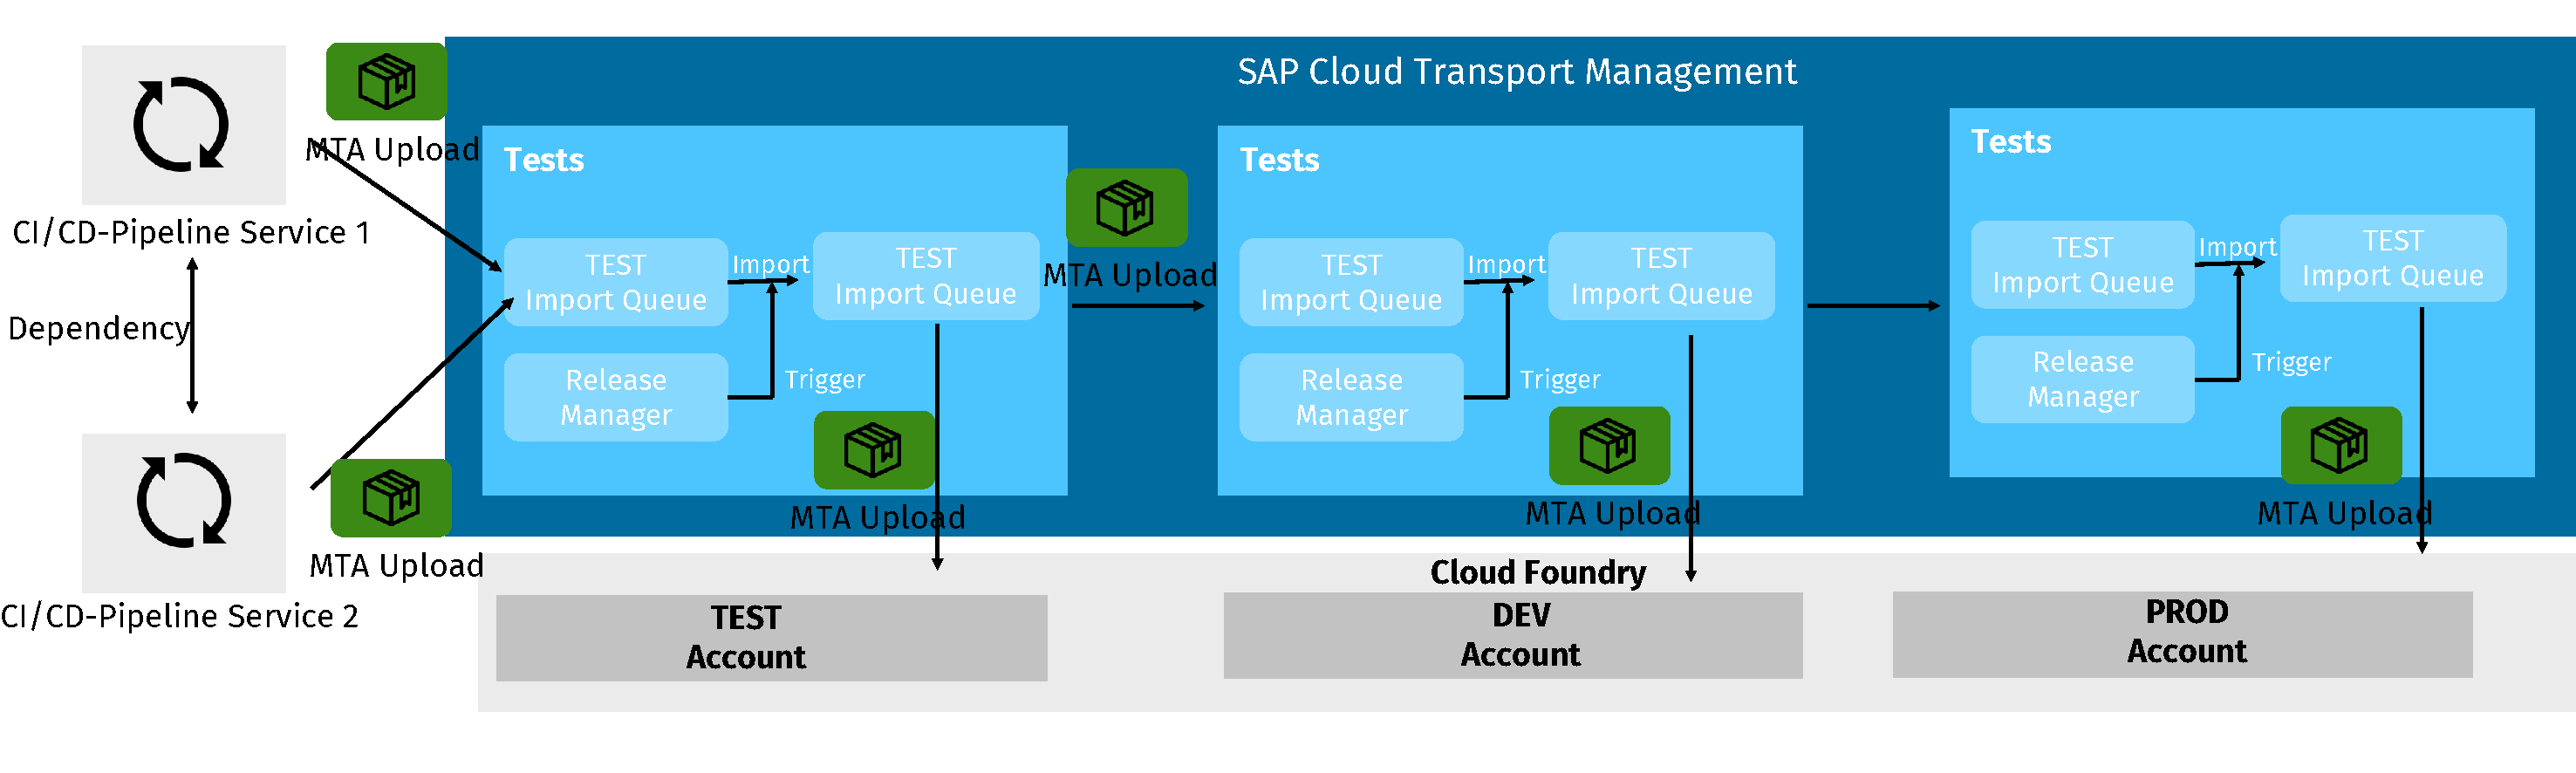
\includegraphics{CTM}}
		\caption[SAP Cloud Transportmanagement]{SAP Cloud Transportmanagement. Eigene Darstellung.}
		\label{fig:CTM}
	\end{figure}
\end{center}
\vspace*{-10mm}In Kategorie K1.5 wird die \textbf{Monitoring-Funktionalität} der verschiedenen CI/CD-Pipelines untersucht. Hierbei wird evaluiert, wie gut ein jeweiliges Tool während des CI/CD-Prozesses überwacht werden kann. Dazu gehört insbesondere die Überwachung des Build-Prozesses. Der fehlerfreie Betrieb soll dabei anhand von sollen Logs oder Metriken wie Build-Zeiten evaluiert werden. Zudem sollte evaluiert werden können, ob alle Tests erfolgreich ausgeführt wurden. Im letzten Schritt des CI/CD-Prozesses soll schließlich ebenfalls die Bereitstellung überwacht werden können. Dabei soll evaluiert werden, ob das Deployment ordnungsgemäß durchgeführt wurde und die Anwendungsstabilität gewährleistet ist.\\
In Kategorie K2 werden die \textbf{Integrationsmöglichkeiten} der Pipeline untersucht. Um auch in diesem Kriterium eine präzise Bewertung zu ermöglichen wird eine Unterteilung in Subkriterien vorgenommen. Dazu gehören die \textit{Integrationsmöglichkeiten von Repositorys} (Kriterium K2.1). Dabei wird evaluiert, ob sich das Repository unmittelbar in die Pipeline integrieren lässt oder ob dies ausschließlich über Webhooks möglich ist. Mit Webhooks können bestimmte Ereignisse, wie das Pushen von Code-Änderungen in einem Repository automatisch an die CI/CD-Pipeline gesendet werden. Somit kann ein unmittelbarer Integrations- bzw. Bereitstellungs-Workflow ausgelöst werden. Da für die Weebhook-Integration manuell eine Schnittstelle aufgesetzt werden muss, ist dies i.d.R. aufwendiger, wie wenn eine unmittelbare Integration in die Pipeline möglich ist. Des Weiteren wird in diesem Kriterium evaluiert, welche Events durch eine Pipeline verarbeitet werden. Besonders vorteilhaft ist, wenn eine Pipeline z.B. Pull-Request-Events verarbeiten kann. So kann sichergestellt werden, dass bevor Änderungen in den Hauptzweig integriert werden, dass keine Konflikte mit dem aktuellen Code auftreten. Bei der Bewertung wird dabei insbesondere evaluiert, dass häufig verwendete Repositorys in die Pipeline integrierbar sind. \\ In Kriterium K1.2 wird evaluiert, ob eine CI/CD-Pipeline ebenfalls in für SAP CAP sowie SAP UI5 kompatible Entwicklungsumgebung integrierbar ist. Dazu gehören Microsoft Visual Studio Code, \ac{SAP BAS} sowie Eclipse. Eine Integration in die Entwicklungsumgebung ermöglicht Programmierern eine höhere Flexibilität bei der Erstellung neuer Funktionalitäten. So kann eine Integration-Pipeline unmittelbar während des Entwicklungsprozesses aus der Entwicklungsumgebung gestartet werden. Dies ermöglicht, dass Entwickler noch schneller Feedback bekommen, wie wenn eine Pipeline ausschließlich in das Repository integrierbar ist.\\
Kriterium K2.3 evaluiert die Integrierbarkeit von Planungssoftware wie Jira. Diese ermöglicht Projektmanager eine höhere Transparenz über den Bereitstellungs-Workflow aller zu implementierender Arbeitselemente zu bekommen. So kann über die Planungssoftware unmittelbar der Build-Status eines neuen Features untersucht werden. Da von der SAP keine Vorgaben bezüglich Planungssoftware getroffen wurden und diese auch unabhängig von dem verwendeten Technologie-Stack ist, wird innerhalb dieses Kriteriums lediglich die generelle Integrierbarkeit von Planungssoftware untersucht.\\ 
In Kriterium K3 erfolgt eine Untersuchung der \textit{Kosten}. Um eine Vergleichbarkeit herzustellen werden die Kosten per Build-Hour verglichen. Da Jenkins auf einem eigenen Server gehostet werden muss, wird evaluiert, wie viele Kosten eine in der Cloud gehostete Instanz verursacht. Zudem wird in einer qualitativen Betrachtung evaluiert, welche Nebenkosten in einer Pipeline jeweils verursacht werden.\\
Das Kriterium K4 untersucht die \textit{Skalierbarkeit} der CI/CD-Pipeline. Dabei wird für die zu untersuchenden Pipelines evaluiert, ob die Möglichkeit einer horizontalen Skalierbarkeit besteht. Dies hat den Vorteil, dass mehrere Builds gleichzeitig durchgeführt werden und die Pipeline somit anhand des Bedarfs gleichzeitiger Builds skaliert werden kann. Zudem wird evaluiert, ob die Ressourcen einer Pipeline-Instanz skaliert werden können. Eine solche vertikale Skalierbarkeit birgt den Vorteil, dass die CI/CD-Pipeline in der Lage ist mit den Anforderungen eins Projektes mitzuwachsen. Dies birgt insbesondere für CEs einen hohen Mehrwert. Mit schnellen und effizienten Entwicklungs- und Bereitstellugnsprozessen können CEs ihre Time-to-Market verkürzen und somit schneller auf die Bedürfnisse der Kunden reagieren.\\
In Kriterium K5 wird die \textit{Performance} der verschiedenen CI/CD-Pipeline verglichen. Dabei wird jedes Tool anhand derselben Anwendung getestet und die Zeit zur Prozessierung des Workflows gemessen. Dabei wird zwischen der Integration- und Delivery-Time unterschieden. Bei der Integration-Time wird die Zeit von der Integration eines Feature-Branchs in den Hauptzweig gemessen. Dabei werden in die Pipelines dem CI-Prozess entsprechende Validierungen, wie Unit- und Integration-Tests eingebaut. Bei der Delivery-Time wird die Zeit die es zur Bereitstellung der Software auf die Cloud-Plattform benötigt bemessen. Dabei werden CD-typische Schritte, wie das Ausführen von Code-Analysen und E2E-Tests implementiert.\\
In Kriterium K6 wird die \textbf{Flexibilität} der verschiedenen Pipelines evaluiert. Dabei wird insbesondere evaluiert, ob die Schritte einer Pipeline uneingeschränkt konfigurierbar sind. So sollte eine sehr flexible Pipeline etwa keine Einschränkungen bezüglich der Anzahl und Reihenfolge von der durchführbaren Tests. Weiterhin wird evaluiert, ob für die Pipeline ein modularer Aufbau möglich ist. Da CEs i.d.R. sehr viele verschiedene Services besitzen, müssen ebenfalls sehr viele Pipelines bereitgestellt werden. Um diese Komplexität zu verringern, sollten eine Pipeline aus modularen und wiederverwendbaren Komponenten bestehen. Wird somit ein neuer Service in die Systemlandschaft integriert können diese Komponenten einfach wiederverwendet werden. Ein weiterer für die Flexibilität der Pipelines essenzieller Aspekt ist die Unterstützung von Plugins. Dies ist gerade für CEs essenziell, da diese mit diesen schnell auf sich ändernde Bedürfnisse reagiert werden kann. Somit können ebenfalls Funktionen in die Pipeline integriert werden, welche sonst im Regelfall nicht standardgemäß verfügbar wären. 
In Kriterium K7 wird der für die CI/CD-Pipelines bereitgestellte \textbf{Support} evaluiert. Hierfür werden entsprechend die Subkriterien \textbf{Administrativer Support} sowie \textbf{Community-Support} definiert. Dabei wird insbesondere untersucht, ob es ein Plattform-Team gibt, welches bei der Einrichtung, Konfiguration sowie Problembehebung der Pipelines unterstützt. Dies ist insbesondere dann hilfreich, wenn die Installierung der Pipeline einen hohen Grad an Expertise benötigt. Des Weiteren wird evaluiert, ob Schulungen sowie Schulungsmaterial verfügbar ist. Dies soll insbesondere unerfahrenen Anwendern bei Nutzung der CI/CD-Pipelines unterstützten. Ein weiterer essenzieller in diesem Kriterium zu beachtender Aspekt ist die Verfügbarkeit von Updates. Werden kontinuierlich Updates an die Anwender ausgeliefert kann sichergestellt werden, dass die Pipeline stets auf dem neusten Stand der Technik ist. Mit Kriterium K7.2, dem Community-Support, wird impliziert, dass es Entwickler gibt, welche sich durch Wartung, Entwicklung und Dokumentation aktiv an der Verbesserung des CI/CD-Services beteiligen. Dabei wird etwa die Verfügbarkeit von Foren evaluiert, in welchen Fragen stellen und Probleme diskutieren können. Neben der Erweiterung der Dokumentation kann eine Community dabei ebenfalls neue Funktionalität für die Pipelines entwickeln.\\
In dem Kriterium K8 wird die Sicherheit der CI/CD-Pipelines untersucht. Hierbei werden die Subkriterien \textit{Authentifizierung und Autorisierung} zur bzw. \textit{Sicherheitsarchitektur} gebildet. In Kriterium K8.1 wird dabei evaluiert, ob eine CI/CD-Pipeline ein Authentifizierungskonzept besitzt. Um unerwünschte Zugriffe zu vermeiden, soll die Verwendung einer Pipeline ausschließlich mit Nutzer-Passwort-Kennung möglich sein. Besonders vorteilhaft ist dabei, wenn zentralisierte Drittanbieter, wie der SAP Identity Provider oder GitHub, als Authentifizierungsmethoden integrierbar sind. Damit kritische Konfiguration ausschließlich von Spezialisten vorgenommen werden, muss eine Pipeline ebenfalls Autentisierungskonzepte unterstützten. Dabei sollen Benutzern über die Implementierung von Rollen bestimmte Rechte eingeräumt werden. In dem Kriterium K8.2, der \textit{Sicherheitsarchitektur}, der Pipeline-Tools untersucht. Zu Erhöhung der Sicherheit ist es z.B. vorteilhaft, wenn CI/CD-Pipelines in isolierten Umgebung, wie z.B. Docker-Container oder virtualisierten Maschinen laufen. Entstehen in der CI/CD-Pipeline Lücken, können sich diese nicht unmittelbar auf andere Systeme ausweiten. Ein weiterer in diesem Kriterium evaluierter Aspekt ist die Ausfallsicherheit. Um sicherzustellen, dass neue Funktionalität bei der Integration kontinuierlich getestet und Software schnell an den Kunden bereitgestellt werden kann, sollten die CI/CD-Systeme hochverfügbar sein.  
\subsection{Entwicklung einer ganzheitlichen Bereitstellungsstrategie}
